% ============================================================
%  TASK 3.1 — ONE-DIODE RECTIFIER TOPOLOGY
%  RF Harvesting Report — Rudkiewicz & Vausort — ESEO 2026
% ============================================================
% Required packages (add to your main preamble if not present):
%   \usepackage{amsmath, amssymb}
%   \usepackage{booktabs}
%   \usepackage{graphicx}
%   \usepackage{siunitx}
%   \usepackage{hyperref}
%   \usepackage{caption}
%   \usepackage{subcaption}
%   \usepackage{float}          % <-- required for [H] float specifier
%
% Also add this in your preamble after \usepackage{siunitx}:
%   \DeclareSIUnit{\dBm}{dBm}
% ============================================================

% ----- If this file is \input directly, uncomment the two lines below -----
% \usepackage{float}
% \DeclareSIUnit{\dBm}{dBm}

\section{Task 3.1 --- One-Diode Rectifier Topology}
\label{sec:task3_1}

This part presents the full characterization of the one-diode rectifier
topology implemented with the HSMS-2860 Schottky diode at an operating
frequency of \SI{2.2}{\giga\hertz}.
The analysis will follow a systematic progression : (1) characterization of the diode
input impedance without any matching network, (2) study of its dependence on
input power and load resistance, (3) design and validation of the lumped-element
impedance matching circuit, (4) extension to a microstrip implementation
including design rule constraints, and (5) evaluation of the one-diode rectifier topology
performance in terms of conversion efficiency~$\eta$, output voltage~$V_\mathrm{out}$,
and output current~$I_\mathrm{out}$.
% ------------------------------------------------------------
\subsection{Diode Input Impedance vs.\ Frequency (without Matching Circuit)}
\label{subsec:zin_vs_freq}
% ------------------------------------------------------------


Before extracting the diode input impedance, it is important to understand the
structure of the one-diode rectifier simulated in ADS, shown in
Figure~\ref{fig:schematic_one_diode}.
The circuit is composed of the following elements:

\begin{itemize}
    \item \textbf{RF source:} a single-tone power source \texttt{P\_1Tone}
          (PORT1, $Z = \SI{50}{\ohm}$) sweeping from \SIrange{1}{3}{\giga\hertz},
          delivering a power $P = \mathrm{polar}(\mathrm{dbmtow}(P_\mathrm{in}), 0)$,
          which converts the input power from dBm to Watts in polar form. It simulates the antenna behavior. 

    \item \textbf{DC-blocking / RF choke network:} two capacitors
      $C_1 = C_2 = \SI{100}{\pico\farad}$ placed in series on the 
      signal path and in shunt at the output respectively.
      $C_1$ blocks any DC component from reaching the source, while 
      $C_2$ shorts the RF signal to ground at the output node, acting 
      as an RF bypass capacitor that forces the load to see only the 
      rectified DC voltage.

    \item \textbf{Schottky diode D1:} the HSMS-2860 model is placed in series between the
          RF input and the output node.
          In this series topology, the diode rectifies the RF signal by conducting
          only during positive half-cycles, charging $C_2$ to a DC voltage.

    \item \textbf{Load resistor:} $R_1 = R_L$, represents the equivalent
          input resistance of tour sensor (STTS22H).
          Here we have, $R_L = \SI{10}{\kilo\ohm}$ for the moment.
\end{itemize}

More on the simulation and measurements parts, we have two current probes (\texttt{I\_Probe1} on the input path, \texttt{I\_Probe2}
on the output path). They are respectively measuring the RF input current and the DC output current. On the other side, 
the LSSP harmonic-balance solver is a linear $S$-parameter
simulation because the diode is a nonlinear component (its behavior
depends on the RF level, this force us large to use signal analysis). Finaly, the impedance $Z_\mathrm{in}$ is extracted via the ADS equation block:
\texttt{Zin1 = zin(S11, PortZ1)}.

\begin{figure}[htbp]
    \centering
    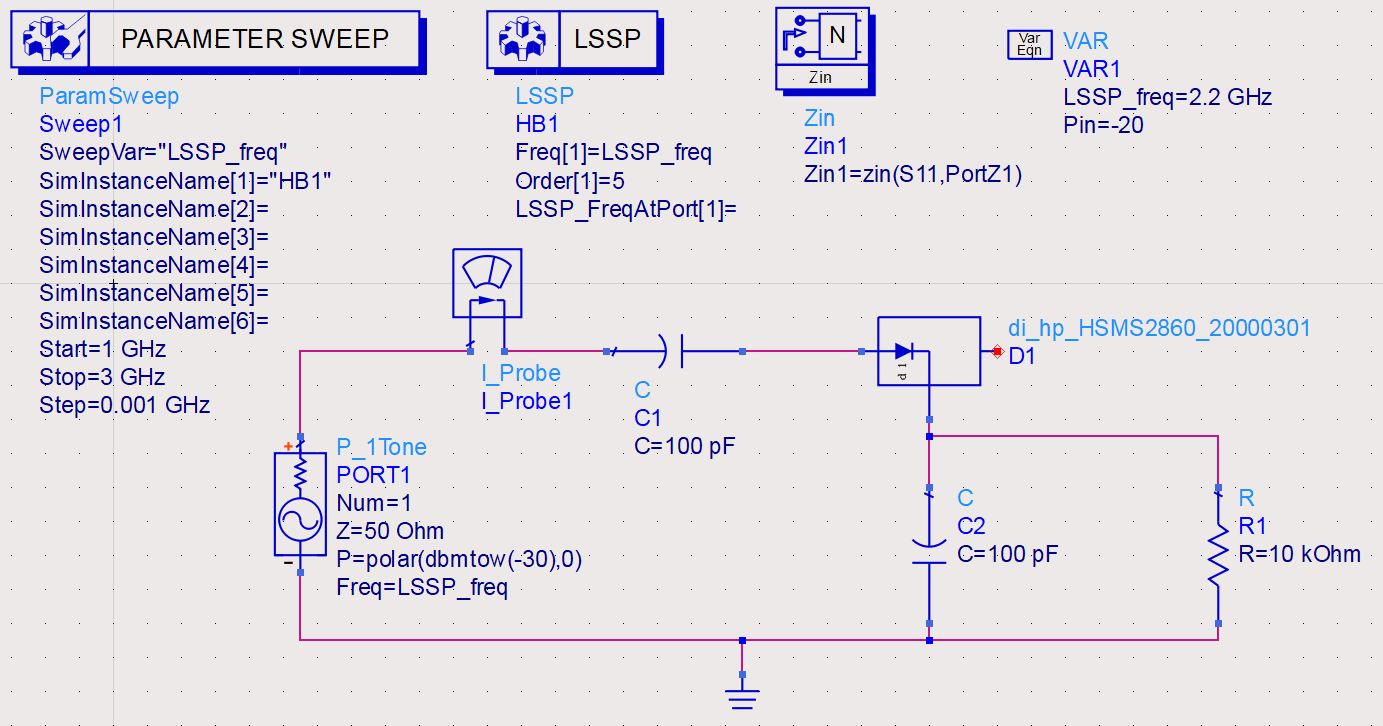
\includegraphics[width=\linewidth]{images/schematic_one_diode.png}
    \caption{ADS schematic of the one-diode series rectifier used for
             input impedance extraction.}
    \label{fig:schematic_one_diode}
\end{figure}

\subsubsection{Simulation setup}

The input impedance $Z_\mathrm{indiode}$ of the HSMS-2860 is extracted using
a LSSP (Large-Signal S-Parameter) simulation in Keysight ADS over the
frequency range \SIrange{1}{3}{\giga\hertz}, with a frequency step of
\SI{1}{\mega\hertz}.
The operating conditions are fixed at $P_\mathrm{in} = -20\,\text{dBm}$ and
$R_L = \SI{10}{\kilo\ohm}$.
The problem is that, the input impedance $Z_\mathrm{in}$ of the diode cannot be measured 
directly in ADS. Instead, the simulator measures the reflection 
coefficient $S_{11}$ at Port~1, which represents the ratio of the 
reflected wave to the incident wave at the port. Since any impedance 
mismatch between the source ($Z_0 = \SI{50}{\ohm}$) and the diode 
causes a partial reflection of the incident signal, $S_{11}$ has 
the full information needed to recover $Z_\mathrm{in}$. The conversion could be done by using this relation:
%
\begin{equation}
    Z_\mathrm{in} = Z_0 \,\frac{1 + S_{11}}{1 - S_{11}},
    \label{eq:zin_from_s11}
\end{equation}
%
which is evaluated in ADS via the built-in function 
\texttt{zin(S11, PortZ1)}.
If $S_{11} = 0$ (no reflection), 
and gives $Z_\mathrm{in} = Z_0 = 
\SI{50}{\ohm}$, confirming perfect matching. On the other hand, if $S_{11} = -1$ 
(total reflection, short circuit), it gives $Z_\mathrm{in} = 0$.

Regarding the two \SI{100}{\pico\farad} capacitors $C_1$ and $C_2$: 
at \SI{2.2}{\giga\hertz}, their impedance is only
$X_C = 1/(2\pi f C) \approx \SI{0.72}{\ohm}$, which is negligible 
compared to $Z_0 = \SI{50}{\ohm}$. Therefore the behave as 
short-circuits at RF frequencies and do not disturb the impedance 
measurement of the diode. At DC, a capacitor blocks any 
current flow, this means that $C_1$ prevents the 
rectified DC voltage from flowing back into the source, and $C_2$ 
ensures that the load $R_L$ receives a clean DC voltage.

% ------------------------------------------------------------
\subsection{Influence of \texorpdfstring{$P_\mathrm{in}$}{Pin} and
            \texorpdfstring{$R_L$}{RL} on \texorpdfstring{$Z_\mathrm{in,diode}$}{Zin}}
\label{subsec:zin_tables}
% ------------------------------------------------------------

\subsubsection{Effect of input power at fixed \texorpdfstring{$R_L = \SI{10}{\kilo\ohm}$}{RL=10kohm}}

The LSSP simulation is repeated for five input power levels
($P_\mathrm{in} \in \{-30, -20, -10, 0, +10\}$\,dBm) with $R_L = \SI{10}{\kilo\ohm}$
fixed.
Table~\ref{tab:zin_vs_pin} summarizes the extracted impedance values at
\SI{2.2}{\giga\hertz}.

\begin{table}[htbp]
    \centering
    \caption{Real and imaginary parts of $Z_\mathrm{in,diode}$ at \SI{2.2}{\giga\hertz}
             for varying $P_\mathrm{in}$, with $R_L = \SI{10}{\kilo\ohm}$.}
    \label{tab:zin_vs_pin}
    \begin{tabular}{S[table-format=-2.0]
                    S[table-format=1.3]
                    S[table-format=-3.3]}
        \toprule
        {$P_\mathrm{in}$ (dBm)} &
        {$\mathrm{Re}(Z_\mathrm{in})$ ($\Omega$)} &
        {$\mathrm{Im}(Z_\mathrm{in})$ ($\Omega$)} \\
        \midrule
        -30 & 2.580 & -259.618 \\
        -20 & 2.533 & -263.520 \\
        -10 & 2.517 & -279.632 \\
          0 & 2.781 & -320.298 \\
         10 & 3.282 & -393.890 \\
        \bottomrule
    \end{tabular}
\end{table}

\paragraph{Analysis.}
Two distinct trends emerge from Table~\ref{tab:zin_vs_pin}:
%
\begin{itemize}
    \item \textbf{Real part:} $\mathrm{Re}(Z_\mathrm{in})$ remains quasi-constant
    across the full power range, varying only from \SI{2.517}{\ohm} to
    \SI{3.282}{\ohm}.
    This is consistent with the physics of the HSMS-2860: the series resistance
    $R_s$ is a bulk property of the metal-semiconductor junction, largely
    independent of the signal level over this range.

    \item \textbf{Imaginary part:} $\mathrm{Im}(Z_\mathrm{in})$ becomes
    increasingly negative as $P_\mathrm{in}$ rises.
    At $P_\mathrm{in} = +10\,\text{dBm}$, the reactance reaches
    $\SI{-393.89}{\ohm}$, compared to $\SI{-259.62}{\ohm}$ at
    $P_\mathrm{in} = -30\,\text{dBm}$.
    This behavior reflects the voltage-dependent nature of the Schottky
    junction capacitance: as the RF voltage swing increases, the average
    junction bias shifts, changing the effective capacitance $C_j(V)$.
\end{itemize}
%
This power-dependency implies that the impedance matching circuit designed for
a specific power level may perform sub-optimally at other power levels.
In a practical low-power RF harvesting scenario ($P_\mathrm{in} \leq -20\,\text{dBm}$),
the variation is small enough to be neglected for a first-order design.

\subsubsection{Effect of load resistance at fixed \texorpdfstring{$P_\mathrm{in} = -20\,\text{dBm}$}{Pin=-20dBm}}

Table~\ref{tab:zin_vs_rl} presents the impedance values for three different
load resistances ($R_L \in \{1, 5, 10\}$\,k$\Omega$) at
$P_\mathrm{in} = -20\,\text{dBm}$.

\begin{table}[htbp]
    \centering
    \caption{Real and imaginary parts of $Z_\mathrm{in,diode}$ at \SI{2.2}{\giga\hertz}
             for varying $R_L$, with $P_\mathrm{in} = -20\,\text{dBm}$.}
    \label{tab:zin_vs_rl}
    \begin{tabular}{S[table-format=2.0]
                    S[table-format=1.3]
                    S[table-format=-3.3]}
        \toprule
        {$R_L$ (k$\Omega$)} &
        {$\mathrm{Re}(Z_\mathrm{in})$ ($\Omega$)} &
        {$\mathrm{Im}(Z_\mathrm{in})$ ($\Omega$)} \\
        \midrule
         1 & 2.522 & -263.520 \\
         5 & 2.522 & -263.520 \\
        10 & 2.522 & -263.520 \\
        \bottomrule
    \end{tabular}
\end{table}

\paragraph{Analysis.}
The impedance is completely insensitive to the load resistance over the range
tested: both $\mathrm{Re}(Z_\mathrm{in})$ and $\mathrm{Im}(Z_\mathrm{in})$
remain strictly constant at \SI{2.522}{\ohm} and \SI{-263.520}{\ohm}
respectively.
This result is physically expected: at RF frequencies (\SI{2.2}{\giga\hertz}),
the LSSP simulation captures the small-signal RF behavior of the diode at its
operating point.
The load resistance $R_L$ only influences the DC bias point of the rectifier
through the output DC voltage, but its effect on the high-frequency
small-signal junction impedance is negligible when $R_L \gg 1/(\omega C_j)$.
Indeed, $1/(\omega C_j) \approx 1/(2\pi \times 2.2 \times 10^9 \times
0.18 \times 10^{-12}) \approx \SI{402}{\ohm}$, which is far smaller than
any of the tested load values.

The key practical implication is that the impedance matching network can be
designed independently of the load resistance for the targeted application
(STTS22H sensor, $R_L \approx \SI{10}{\kilo\ohm}$), which simplifies the
design process considerably.

% ------------------------------------------------------------
\subsection{Lumped-Element Impedance Matching Circuit}
\label{subsec:matching_lumped}
% ------------------------------------------------------------

\subsubsection{Design methodology}

The objective of the matching network is to transform the antenna source
impedance $Z_0 = \SI{50}{\ohm}$ to the complex conjugate of the diode input
impedance $Z_\mathrm{in,diode}^*$, so as to maximize power transfer.
The design employs the ADS dynamic tuning tool (\emph{Tune}) to iteratively
adjust the component values while observing $S_{11}$ and $Z_\mathrm{in}$
in real time.
The target specification is:
%
\begin{equation}
    S_{11}(f = \SI{2.2}{\giga\hertz}) < \SI{-10}{\deci\bel}.
    \label{eq:s11_spec}
\end{equation}

The matching topology selected is a two-stage LC ladder network inserted
between the RF port and the diode.
This topology uses the following real SMD components:
%
\begin{itemize}
    \item Two shunt capacitors: $C_7 = \SI{3.3}{\pico\farad}$ and
          $C_8 = \SI{3.9}{\pico\farad}$ (series UPY-AQ NP0, 16--50\,V);
    \item Two series inductors: $L_2 = \SI{18}{\nano\henry}$ and
          $L_3 = \SI{8.2}{\nano\henry}$.
\end{itemize}
%
All components are modeled in ADS using their $\mathrm{C\_Pad1}$ and
$\mathrm{L\_Pad1}$ footprint models (0603 SMD package), which include the
parasitic elements associated with the physical pad geometry:
$W = \SI{0.8}{\milli\meter}$, $S = \SI{0.4}{\milli\meter}$,
$L_1 = \SI{1.6}{\milli\meter}$ for the capacitors, and
$W = \SI{0.64}{\milli\meter}$, $S = \SI{0.56}{\milli\meter}$,
$L_1 = \SI{1.19}{\milli\meter}$ for the inductors.

\subsubsection{Results after tuning}

After optimization, the resulting impedance at \SI{2.2}{\giga\hertz} is:
%
\begin{align}
    \mathrm{Re}(Z_\mathrm{in})\big|_\mathrm{matched}
        &= \SI{48.652}{\ohm}, \\
    \mathrm{Im}(Z_\mathrm{in})\big|_\mathrm{matched}
        &= \SI{-10.990}{\ohm}.
\end{align}
%
The optimal tuning values found by the ADS Tune tool are
$\mathrm{Cap} = \SI{7.286}{\pico\farad}$ and
$\mathrm{Ind} = \SI{26.247}{\nano\henry}$, which guided the selection of
the nearest standard commercial values ($C_7 = \SI{3.3}{\pico\farad}$,
$C_8 = \SI{3.9}{\pico\farad}$, $L_2 = \SI{18}{\nano\henry}$,
$L_3 = \SI{8.2}{\nano\henry}$).

The $S_{11}$ parameter of the matched circuit reaches
\textbf{\SI{-21.84}{\deci\bel}} at \SI{2.2}{\giga\hertz}, as shown in
Figure~\ref{fig:s11_matched_lumped}, which satisfies the specification
of~(\ref{eq:s11_spec}) with a margin of more than \SI{11}{\deci\bel}.

\begin{figure}[htbp]
    \centering
    % \includegraphics[width=0.75\linewidth]{figures/s11_matched_lumped.png}
    \caption{$S_{11}$ parameter of the one-diode rectifier with the
             lumped-element matching circuit ($C_7 = 3.3$\,pF,
             $C_8 = 3.9$\,pF, $L_2 = 18$\,nH, $L_3 = 8.2$\,nH).
             $R_L = 10$\,k$\Omega$, $P_\mathrm{in} = -20$\,dBm.
             Marker m3: $S_{11}(2.2\,\mathrm{GHz}) = -21.84$\,dB.}
    \label{fig:s11_matched_lumped}
\end{figure}

\subsubsection{Asymmetry of the \texorpdfstring{$S_{11}$}{S11} response}

A notable feature of the $S_{11}$ curve in Figure~\ref{fig:s11_matched_lumped}
is its pronounced \emph{asymmetry} around the resonance frequency.
The response rises steeply on the low-frequency side and rolls off more
gradually on the high-frequency side, rather than presenting a symmetric
band-pass shape.

This asymmetry is a direct consequence of using a \textbf{single diode}
topology.
The Schottky diode acts as a nonlinear, non-reciprocal element: it conducts
preferentially during positive half-cycles of the RF signal, creating a
half-wave rectification process.
This introduces even-order harmonic distortion and a DC offset that modulates
the effective junction impedance differently on each side of resonance.
In a two-diode topology (voltage doubler), the two diodes conduct on opposite
half-cycles, and their nonlinear contributions cancel to first order, restoring
a more symmetric $S_{11}$ profile.
This difference will be examined further in the comparative analysis of
Section~\ref{sec:task4}.

% ------------------------------------------------------------
\subsection{Extension to Microstrip Implementation}
\label{subsec:matching_microstrip}
% ------------------------------------------------------------

\subsubsection{Substrate and design rules}

The physical PCB implementation follows the design rules specified for this
project:
%
\begin{itemize}
    \item Substrate: Rogers 4350B ($\varepsilon_r = 4.5$,
          $\tan\delta = 0.02$, $H = \SI{1.6}{\milli\meter}$,
          copper thickness $T = \SI{0}{\milli\meter}$ in ADS model);
    \item Signal traces: characteristic impedance $Z_0 = \SI{50}{\ohm}$,
          corresponding to $W = \SI{3.034}{\milli\meter}$;
    \item Microstrip line length constraints:
          $\SI{3}{\milli\meter} \leq L_\mathrm{line} \leq \SI{10}{\milli\meter}$;
    \item SMD package: 0603.
\end{itemize}
%
Each lumped component (capacitor, inductor) is surrounded by two MLIN
microstrip segments on either side, connected through MTEE-ADS T-junction
elements to model the physical routing on the PCB.
All line segments use $W = \SI{3.034}{\milli\meter}$, consistent with
$Z_0 = \SI{50}{\ohm}$.

\subsubsection{Effect of microstrip parasitics on resonance frequency}

When the MLIN segments are introduced into the simulation while keeping
the original lumped component values unchanged ($C_7 = \SI{3.3}{\pico\farad}$,
$C_8 = \SI{3.9}{\pico\farad}$, $L_2 = \SI{18}{\nano\henry}$,
$L_3 = \SI{8.2}{\nano\henry}$), the $S_{11}$ resonance shifts from
\SI{2.2}{\giga\hertz} to approximately \SI{1.8}{\giga\hertz}
(Figure~\ref{fig:s11_microstrip_initial}).
The degradation is caused by the additional inductance and capacitance
contributed by the microstrip lines, which effectively increase the total
reactive energy stored in the network.
A re-tuning of the matching circuit is therefore required to restore the
resonance at the target frequency.

\begin{figure}[htbp]
    \centering
    % \includegraphics[width=0.75\linewidth]{figures/s11_microstrip_initial.png}
    \caption{$S_{11}$ of the lumped matching circuit with MLIN microstrip
             segments added, before re-tuning. The resonance dip shifts to
             approximately 1.8\,GHz due to parasitic contributions of
             the transmission line segments.}
    \label{fig:s11_microstrip_initial}
\end{figure}

\subsubsection{Simplified 1C--1L topology with re-tuning}

To reduce design complexity and component count, the two-stage LC ladder is
simplified to a single shunt capacitor and a single series inductor.
A parameter sweep in ADS over the line length $L$, the capacitance
$\mathrm{Cap}$, and the inductance $\mathrm{Ind}$ yields the following
optimal values:
%
\begin{equation}
    L = \SI{4.19}{\milli\meter}, \quad
    C = \SI{39}{\pico\farad}, \quad
    L_\mathrm{ind} = \SI{2.7}{\nano\henry}.
    \label{eq:opt_1c1l}
\end{equation}
%
With these values, the $S_{11}$ achieves:
%
\begin{align}
    S_{11}(f = \SI{2.200}{\giga\hertz}) &= \SI{-31.37}{\deci\bel}
        \quad (\text{marker m1}), \\
    S_{11}(f = \SI{2.208}{\giga\hertz}) &= \SI{-15.41}{\deci\bel}
        \quad (\text{marker m2}).
\end{align}
%
The result is shown in Figure~\ref{fig:s11_1c1l_retuned}.
The specification $S_{11} < \SI{-10}{\deci\bel}$ is satisfied over a
bandwidth of approximately \SI{35}{\mega\hertz} centered on \SI{2.2}{\giga\hertz},
confirming that the simplified topology is well adapted after re-tuning.

\begin{figure}[htbp]
    \centering
    % 
\includegraphics[width=0.75\linewidth]{figures/s11_1c1l_retuned.png}
    \caption{$S_{11}$ of the simplified 1C--1L matching circuit with
             microstrip segments, after parameter sweep re-tuning.
             $L = 4.19$\,mm, $C = 39$\,pF, $L_\mathrm{ind} = 2.7$\,nH.
             m1: $S_{11}(2.200\,\mathrm{GHz}) = -31.37$\,dB;
             m2: $S_{11}(2.208\,\mathrm{GHz}) = -15.41$\,dB.}
    \label{fig:s11_1c1l_retuned}
\end{figure}

\subsubsection{Fully distributed microstrip implementation}

As a final step, the lumped capacitor and inductor are replaced by
microstrip stubs acting as distributed reactive elements.
This topology is more suitable for monolithic or low-profile PCB integration
and eliminates the dependency on lumped SMD components.
The full set of tuning parameters and their optimal values after the ADS
Tune optimization are listed in Table~\ref{tab:microstrip_only_tune}.

\begin{table}[htbp]
    \centering
    \caption{Optimized parameter values for the fully distributed microstrip
             matching network (one-diode topology, \SI{2.2}{\giga\hertz}).}
    \label{tab:microstrip_only_tune}
    \begin{tabular}{lll}
        \toprule
        Parameter & Physical meaning & Optimized value \\
        \midrule
        $W_C$ & Width of capacitive stub      & \SI{0.56}{\milli\meter} \\
        $L_C$ & Length of capacitive stub     & \SI{1.8}{\milli\meter} \\
        $L_L$ & Length of inductive stub      & \SI{7.6}{\milli\meter} \\
        $W_L$ & Width of inductive stub       & \SI{1.32}{\milli\meter} \\
        $L$   & Main line segment length      & \SI{4.12}{\milli\meter} \\
        Cap   & Residual lumped capacitance   & \SI{39}{\pico\farad} \\
        Ind   & Residual lumped inductance    & \SI{2.7}{\nano\henry} \\
        \bottomrule
    \end{tabular}
\end{table}

With this fully distributed configuration, the $S_{11}$ reaches
\textbf{\SI{-40.84}{\deci\bel}} at \SI{2.2}{\giga\hertz}
(Figure~\ref{fig:s11_microstrip_only}), representing the best matching
performance achieved in this study.
The very deep and narrow resonance is characteristic of a high-$Q$ network,
which maximizes power transfer at the design frequency at the cost of a
reduced matching bandwidth.
For the targeted ISM-band application at \SI{2.2}{\giga\hertz}, this
trade-off is acceptable given that the ambient RF source (Wi-Fi, cellular)
is narrowband.

\begin{figure}[htbp]
    \centering
    % \includegraphics[width=0.75\linewidth]{figures/s11_microstrip_only.png}
    \caption{$S_{11}$ of the fully distributed microstrip matching network
             (one-diode topology).
             Marker m1: $S_{11}(2.200\,\mathrm{GHz}) = -40.84$\,dB.
             The $-10$\,dB bandwidth is approximately 30\,MHz.}
    \label{fig:s11_microstrip_only}
\end{figure}

% ------------------------------------------------------------
\subsection{Rectifier Performance: \texorpdfstring{$\eta$}{eta},
            \texorpdfstring{$V_\mathrm{out}$}{Vout},
            \texorpdfstring{$I_\mathrm{out}$}{Iout}}
\label{subsec:performance}
% ------------------------------------------------------------

The RF-to-DC power conversion efficiency is defined as:
%
\begin{equation}
    \eta = \frac{P_\mathrm{DC}}{P_\mathrm{RF}}
         = \frac{V_\mathrm{out} \cdot I_\mathrm{out}}{V_\mathrm{in} \cdot I_\mathrm{in}}
         \times 100\,\%.
    \label{eq:pce}
\end{equation}

\subsubsection*{Note on figures}
The curves for $\eta$, $V_\mathrm{out}$ and $I_\mathrm{out}$ as a function
of (a)~$R_L$ and (b)~$P_\mathrm{in}$, both with and without microstrip lines,
are to be inserted here as Figures~\ref{fig:perf_vs_rl} and~\ref{fig:perf_vs_pin}
once the ADS transient or harmonic-balance simulations are completed.

\begin{figure}[htbp]
    \centering
    % \includegraphics[width=\linewidth]{figures/perf_vs_rl.png}
    \caption{Rectifier performance ($\eta$, $V_\mathrm{out}$, $I_\mathrm{out}$)
             as a function of load resistance $R_L$
             (\SIrange{1}{10}{\kilo\ohm}), with and without microstrip lines.
             $P_\mathrm{in} = -20$\,dBm, $f = 2.2$\,GHz.}
    \label{fig:perf_vs_rl}
\end{figure}

\begin{figure}[htbp]
    \centering
    % \includegraphics[width=\linewidth]{figures/perf_vs_pin.png}
    \caption{Rectifier performance ($\eta$, $V_\mathrm{out}$, $I_\mathrm{out}$)
             as a function of input power $P_\mathrm{in}$
             (-20 to 10\,\text{dBm}), with and without microstrip lines.
             $R_L = 10$\,k$\Omega$, $f = 2.2$\,GHz.}
    \label{fig:perf_vs_pin}
\end{figure}

\subsubsection{Adequacy for powering the STTS22H sensor}

The STTS22H temperature sensor requires a supply voltage between \SI{1.5}{\volt}
and \SI{3.6}{\volt} and a supply current below \SI{120}{\micro\ampere}.
At an input power of $P_\mathrm{in} = +10\,\text{dBm}$ (the maximum considered
in this study), the one-diode rectifier must provide at least:
%
\begin{equation}
    P_\mathrm{DC,min}
    = V_\mathrm{DD,min} \times I_\mathrm{DD,max}
    = 1.5 \times 120 \times 10^{-6}
    = \SI{180}{\micro\watt}.
\end{equation}
%
Whether this threshold is met depends on the PCE achieved at $+10\,\text{dBm}$,
which will be quantified from the simulation curves of
Figure~\ref{fig:perf_vs_pin}.
The answer to this question will be provided upon completion of the transient
simulation.